\documentclass[a4paper, 12pt]{article}
\usepackage[english]{babel}
\usepackage[numbers]{natbib}
\usepackage{url}
\usepackage[utf8x]{inputenc}
\usepackage{amsmath}
\usepackage{graphicx}
\graphicspath{{figures/}}
\usepackage{parskip}
\usepackage{fancyhdr}
\usepackage{vmargin}
\usepackage{amsmath,amsfonts,amssymb,amsthm,epsfig,epstopdf,titling,url,array}
\theoremstyle{definition}
\newtheorem{definition}{Definition}[section]
\newtheorem{conj}{Conjecture}[section]
\newtheorem{exmp}{Example}[section]
\setmarginsrb{2.5 cm}{2.5 cm}{2.5 cm}{2 cm}{1 cm}{1 cm}{1 cm}{1.5 cm}

\title{\Large Analysis of Injection Attack on SVD-based Collaborative Filtering Algorithm}     % Title
\author{}                               % Author
\date{\today}                                           % Date

\makeatletter
\let\thetitle\@title
\let\theauthor\@author
\let\thedate\@date
\makeatother

\pagestyle{fancy}
\fancyhf{}
\rhead{\theauthor}
\lhead{\thetitle}
\cfoot{\thepage}

\usepackage{amsmath}
\usepackage{float}
\usepackage{listings}
\usepackage{xcolor}
\usepackage{float}

\begin{document}

\begin{titlepage}
    \centering
    \vspace*{0.5 cm}
    
\includegraphics[scale = 0.4]{sustech_logo.png}\\[1.0 cm]   % University Logo
    \textsc{\Large Southern University of Science and Technology}\\[1.5 cm]   % University Name             
    \textsc{\large Course Name:Advanced computer science experiment}\\[0.5 cm]               % Course Name
    \rule{\linewidth}{0.2 mm} \\[0.5 cm]
    { \huge \bfseries \thetitle}\\
    \rule{\linewidth}{0.2 mm} \\[1.5 cm]
    
    \begin{minipage}{0.4\textwidth}
        \begin{flushleft} \large
            \emph{Author:}\\
            
            \theauthor
            \emph{Mentor:}\\
            \end{flushleft}
            \end{minipage}~
            \begin{minipage}{0.4\textwidth}
            \begin{flushright} \large
            \emph{Student Number:} \\
            \emph{E-mail:}\\               
        \end{flushright}
    \end{minipage}\\[2 cm]
    
    {\large \thedate}\\[2 cm]
 
    \vfill
    
\end{titlepage}

%%%%%%%%%%%%%%%%%%%%%%%%%%%%%%%%%%%%%%%%%%%%%%%%%%%%%%%%%%%%%%%%%

\tableofcontents
\pagebreak

%%%%%%%%%%%%%%%%%%%%%%%%%%%%%%%%%%%%%%%%%%%%%%%%%%%%%%%%%%%%%%%%%

\section{Research Background}
\paragraph{}Collaborative filtering(CF) algorithm is the most basic kind of algorithms in recommender system field. It is widely used in e-commerce, like Amazon. There are three kinds of collaborative filtering algorithms: user-based CF, item-based CF and model-based CF. In the second phase of the project, we have implemented a user-based CF recommender system and a SVD-based CF recommender system which is a kind of model-based CF recommender system. 
\paragraph{}In the e-commerce competition, some intentional users inject a large number of falsified data in order to safeguard their own interests. Under such disturbances, the accuracy of recommender system decreases. Therefore, it is important to do research on the attack behavior of collaborative filtering recommender systems. Thus the research of Lam[1] got a result that item-based CF algorithm is more robust than user-based CF algorithm, the focus of our work is on attack behaviors to the SVD-based recommender system. We hack the system with random attack, mean attack and love/hate attack, then analize their effects on the SVD-based recommender system.



\section{SVD-based Collaborative Filtering Algorithm}

The data matrix of $user\quad and\quad item$ is huge.  And there are many blanks in this matrix,  so it is also an extrmely sparse matrix.  We defined this scoring matrix as $R_{U\times I}$
\begin{table}[H]
	\label{user/item matrix}
	\caption{user/item matrix}
	\centering
	\begin{tabular}{|c|c|c|c|c|c|}
		\hline 
		user/item&1&2&3&4&$\cdots$ \\ \hline
		1&5&4&4.5&?&$\cdots$ \\ \hline
		2&?&4.5&?&4.5&$\cdots$\\ \hline
		3&4.5&?&4.4&4&$\cdots$\\ \hline
		$\cdots$&$\cdots$&$\cdots$&$\cdots$&$\cdots$ &$\cdots$ \\ \hline
	\end{tabular}
\end{table} 
The scoring matrix $R_{U\times I}$ can be decompesed as two matrices$P$ and $Q$:
\begin{equation}
R_{U \times I}=P_{U\times k}Q_{k\times I}
\end{equation}
$U$ is the number of users,  $I$ is the number of items,  $k$ is the rank of matrix $R$.\\
Assuming that the known score is $r_{ui}$,  the error between the true value and the predicted value is:
\begin{equation}
e_{ui}=r_{ui}-{\widehat{r}}_{ui}
\end{equation} 
The total error squared sum is:
\begin{equation}
SSE=\sum_{u,i}{e_{ui}}^{2}=\sum_{u,i}(r_{ui}-\sum_{k=1}^{K}p_{uk}q_{ki})
\end{equation}
\subsection{Basic SVD with Gradient Descent}
\begin{equation}
\begin{split}
\frac{\partial }{\partial p_{uk}}SSE&=\frac{\partial}{\partial p_{uk}}\sum_{u,i}(e_{ui})^{2}\\
&=2e_{ui}\frac{\partial}{\partial p_{uk}}e_{ui}\\
&=2e_{ui}\frac{\partial}{\partial p_{uk}}(r_{ui}-\sum_{k=1}^{K}p_{uk}q_{ki})\\
&=2e_{ui}q_{ki}
\end{split}
\end{equation}
Explanation for the equation:\\
there is no summary symbol in the second step because only the equation which has $u$ has the derivative result,  other equations' derivative results are zero.
\begin{equation}
\begin{split}
p_{uk}:=p_{uk}-\eta(-e_{ui}q_{ki})=p_{uk}+\eta e_{ui}q_{ki}\\
q_{ki}:=q_{ki}-\eta(-e_{ui}p_{uk})=q_{ki}+\eta e_{ui}p_{uk}
\end{split}
\end{equation}
There are two different ways to update the two arguments:
\begin{itemize}
	\item \textbf{Batch Gradient Descent Algorithm}\\
	Update $p$,$q$ after calculating all the predictions of known scores
	\item \textbf{Random Gradient Descent Algorithm}\\
	Update $p$,$q$ after calculating one $e_{ui}$	
\end{itemize}
We choose random gradient descent algorithm because we have to minimize the equation $SSE$,  so we have to search in the direction of negative gradient, this may cause the gradient descent stop in the local optimal solution if we use bath gradient descent algorithm. 
\subsection{Adding Biases}
The equation 17 complains the interactions between users and items that produce the different rating values. However, much of the ovserved variation in rating values is due to effects associated with either users or items, known as biases or intercepts.

A first-order approximation of the bias involved in ranting $r_{ui}$ is as follows:
\begin{equation}
b_{ui}=\mu+b_i+b_u
\end{equation}
$b_{ui}$ is the estimation of the rank the user may gives. $\mu$ is the mean of all the item ranks, $b_u$ is the user's mean rank and $b_i$ is the mean rank that the item gets.
\begin{equation}
\hat{r_{ui}}=\mu +b_i+b_u+{q_i}^Tp_{u}
\end{equation}
\subsection{Gradient Descent with Biases}
As users ratings of the merchandise not only depends on a relationship between users and products, but also depends on the unique properties of the users and products.
\begin{equation}
\begin{split}
SSE&=\frac{1}{2}(\sum_{u,i}{e_{ui}}^2+\lambda \sum_{u}|p_u|+\lambda \sum_{i}|q_i|+\lambda \sum_u {b_u}^2+\lambda \sum_u{b_i}^2)\\
&=\frac{1}{2}\sum_{u,i}(r_{ui}-\mu-b_u-b_i-\sum_{k=1}^{K}p_{uk}q_{ki})^2+\frac{1}{2}(\lambda \sum_{u}|p_u|+\lambda \sum_{i}|q_i|+\lambda \sum_u {b_u}^2+\lambda \sum_u{b_i}^2)
\end{split}
\end{equation}
\begin{equation}
\begin{split}
\frac{\partial }{\partial b_{u}}SSE&=-e_{ui}+\lambda b_u \\
\frac{\partial }{\partial b_{i}}SSE&=-e_{ui}+\lambda b_i 
\end{split}
\end{equation}
Then implies the equation to update $b_u$ and $b_i$:
\begin{equation}
\begin{split}
b_u := b_u +\eta(e_{ui}-\lambda b_u)\\
b_i := b_i +\eta(e_{ui}-\lambda b_i)
\end{split}
\end{equation}


The details of the algorithm is as follows:\\


Firstly, generate two random value matrix p and q, then use gradient descent to minimize the error and update $b_i$, $b_u$, p, and the mean-square error Rmse.\\


If Rmse increase, it means that the result just strides the local optimal point. So the train process has been finished.\\


The return result is the matrix p and q.\\


\textbf{The explaination of some variables:} 
\begin{itemize}
	
	\item iteration\_times: the iteration times that gradient descent runs
	\item $b_u$: mean rank of a user gives
	\item $b_i$: mean rank that a product gets
	\item e: error
	\item eta: gradient descent step length, when the result is close local optimal result, we should decrease the step length 
	\item l: regularization parameter
\end{itemize}

\section{Injection Attacks}
\paragraph{}Injection attack indicates that attackers make the recommendation results biased through injecting falsified users into recommender systems. A User Profile is an n-dimendion vector $UP_i = (r_1,r_2,r_3,\cdots,r_n)$ where n is the number of all items in the system. Denote I as the item set of a recommender system and $I = I_T \ I_S \cup I_F \cup I_{\varnothing}$ where $I_T$ is target items, $I_S$ is a set of items specified to improve the efficiency of the attack, $I_F$ is the set of items that need to be assigned a rating and $I_{\varnothing}$ is an unrated set of items. Hence, $Attack = (UP_1, UP_2, UP_3,\cdots, UP_{m-1})$.
\paragraph{}There are four types of injection attack: basic attack, low-acknowledge attack, nuke attack and informed attack[2].
\begin{itemize}
	\item Basic attack
	\begin{itemize}
		\item Random attack\\
		Random attack is to select the user data of a certain fill size after the attacker determines the attack target, then scores the highest score or lowest score for the target items and scores the items in the $I_F$ randomly within a small range centered on the average value of all users for all the items. The average rating of all items by all users in many systems is public and the attacker can get this information, so the cost of knowledge for random attacks is minimal and realistically feasible.
		\item Mean attack\\
		The mean attack is basically the same as the random attack. The  difference is that the evaluation value of the item $i$ in the $I_F$ set is randomly selected within a very small range centered on the average evaluation value of the item $i$ by all the users. Its knowledge cost is high. It needs to know the average of all projects and it is difficult to achieve.
	\end{itemize}
	\item Low-acknowledge attack
	\begin{itemize}
		\item Bandwagon attack\\
		Bandwagon attack binds the target items with a small amount of popular items which have a large number of user groups. Therefore, the target items is more likely to be recommended.
		\item Segment attack\\
		Segment attack recommends target items to specific user groups. Attackers often bind the target items with the popular items that these users like. Therefore, the recommendation algorithm can easily recommend the target product to these user groups.
	\end{itemize}
	\item Nuke attack
	\begin{itemize}
		\item Love/hate attack\\
		It simply gives the highest score for those target items and the lowest score for those products that need to be filtered. This attack requires a very little bit of information, but it is very effective for user-based collaborative filtering algorithms.
		\item Reverse Bandwagon attack\\
		It is a variation of the Bandwagon attack. Unlike the Bandwagon attack, those target items are often tied to very unpopular items in the system. In this case, the system cannot easily recommend those target items.
	\end{itemize}
	\item Informed attack
	\begin{itemize}
		\item Popular attack\\
		It is for user-based CF algorithm. It needs more information, including the recommendation algorithm, the average score of the product, and the user's average score, because the similarities of users do not depend on the co-rated item number in practice and the Pearson correlation coefficient may be negative.Popular attack uses the average score of all items. According to whether the item's score is higher than the average, the item is rated $r_{min+1}$ and $r_{min}$, where $r_{min}$ represents the lowest score. Then, the Pearson correlation coefficient of falsified users and original users has a big probability to be positive, which means the predicted scores of target items are likely to be higher.
		\item Probe Attack Strategy\\
		Probe attack strategy is harder to detect than popular attack. It fakes a user first, then the system will recommend some items for it. With this recommendation information, we have some knowledge about its neighbors. Then we can attack the neighbors with other attack methods.
	\end{itemize}
\end{itemize}


\section{Evaluation}
\paragraph{}For the TopN recommended system, the  Average Hit Ratio Difference is used to evaluate the attack efficiency. Hit ratio is the percentage of the hit number of predicted item and the total number of items of the user in the TopN results of the target item $i$ in the test set. $R_u$ is the TopN item set the system recommended to the user $u$, $H_{ui}=1$ means item $i\in R_u$ otherwise $H_{ui}=0$. Test set $U$ defines the average hit ratio of push attacks on item $i$ is $HitRatio_i=\sum_{u\in U}H_{ui}/|U|$. Similarly, the average hit ratio diffenence $AHitRatio_i=\sum_{i\in I}HitRatio_i/|I|$.
\paragraph{}In our experiment, we do not classify the category of the movies. We do not know the users' favorite movie category. So we can only choose three of the injection attacks: random attack, average attack and love/hate attack. We use AHRD as our evaluation criteria.
\begin{equation}
f(x\mid\mu,b) = \frac{1}{2b} \exp \left( -\frac{|x-\mu|}{b} \right)
\end{equation}
\begin{figure}[H]
	\centering
	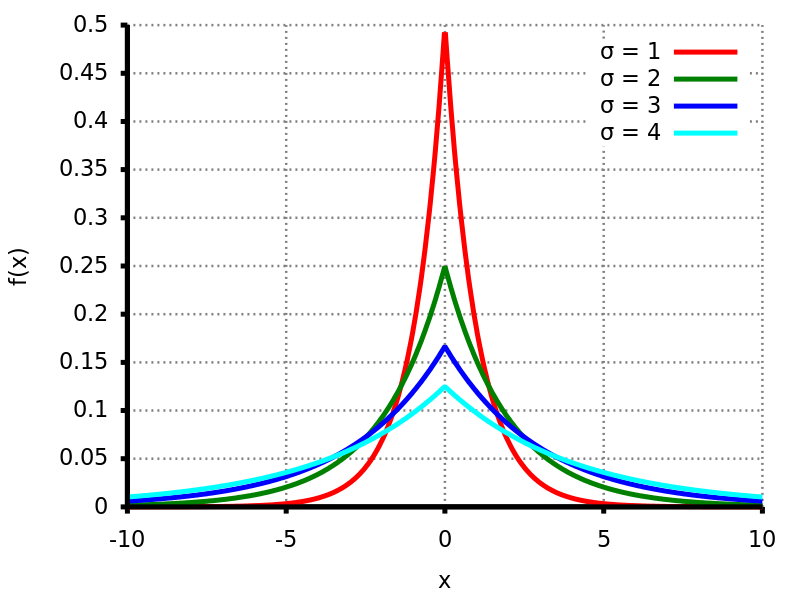
\includegraphics[scale = 0.4]{Laplace.png}
	\caption{Laplace distribution}
\end{figure}
\paragraph{} We add Laplace noises to the original data which arugument b=1,2,3,4,5,6.\\


For the three attacks:
\begin{itemize}
	\item Average Attack:\\
	 \begin{itemize}
	 	\item Random pick 5 movies(objective movies) and random pick 100 users(the attackers).
	 	\item These 100 users give the ovjective movies rank 5 and every users choose random 5 movies to give the average rank other users given.
	 \end{itemize}
 	\item Random Attack:\\
 \begin{itemize}
 	\item Random pick 5 movies(objective movies) and random pick 100 users(the attackers).
 	\item These 100 users give the ovjective movies rank 5 and every users choose random 5 movies to give the random rank range 0 to 5.
 \end{itemize}
\item Love/hate Attack:\\
\begin{itemize}
	\item Random pick 5 movies(objective movies) and random pick 100 users(the attackers).
	\item These 100 users give the ovjective movies rank 5 and do not rank other movies.
\end{itemize}
\end{itemize}
\section{Result and Analysis}
\subsection{Result}
The running result of our experiment.
\begin{figure}[H]
	\centering
	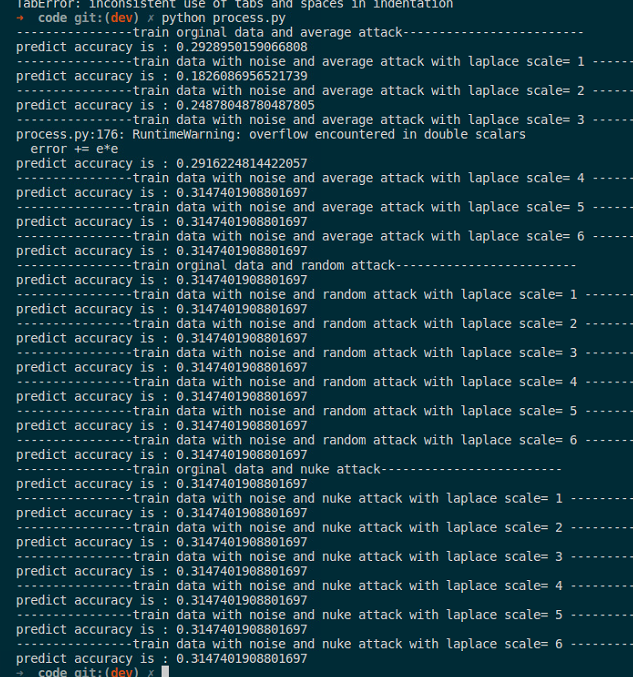
\includegraphics[scale = 0.4]{result.png}
	\caption{The result}
\end{figure}
The average hit ratio with noise(b=1,2,3,4,5,6)
\begin{figure}[H]
	\centering
	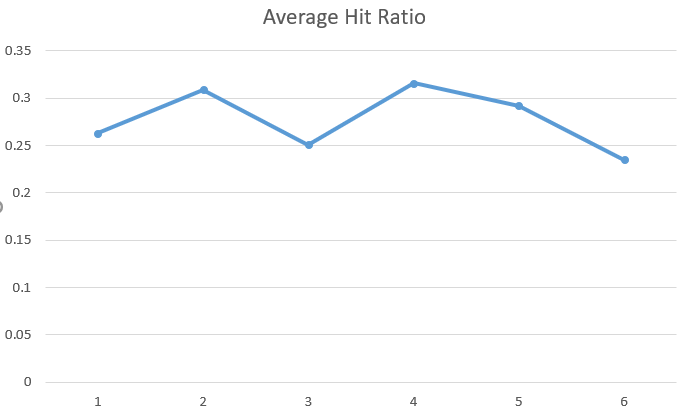
\includegraphics[scale = 0.4]{hit-ratio.png}
	\caption{AHR with noise}
\end{figure}
The average hit ratio with attacks:
\begin{figure}[H]
	\centering
	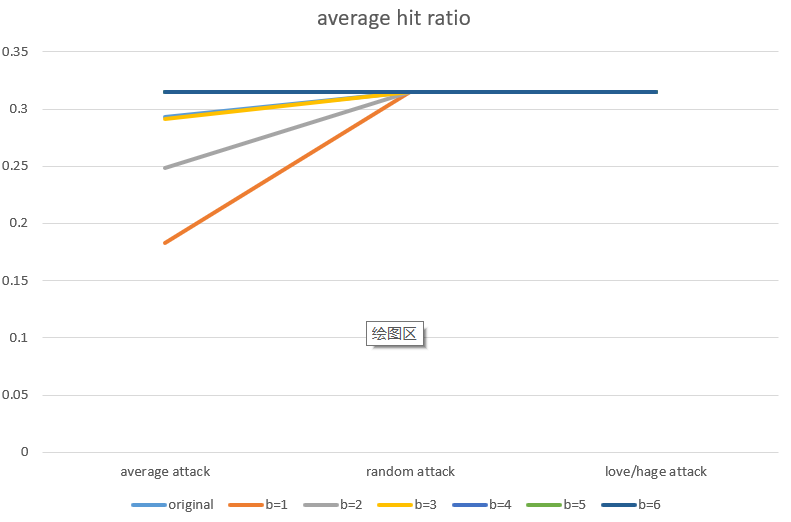
\includegraphics[scale = 0.4]{hit-ratio-attack.png}
	\caption{AHR with attacks}
\end{figure}
\subsection{Analysis}
\paragraph{}According to the experiment result, when b is increase, the result efficiency is increasing during some time, but when b is large than 4, then result efficiency is dereasing. Because when b=1, the Laplace noise is too harsh in the middle, it may influence some specific users, and then derease the prediction ratio. When b is too large(large than 5), almost every user is influenced by the noise, the prediction ratio is decreasing.
\paragraph{}When we simulate some injection into the recommend system, the result does not influenced by the random attack and love/hate attack, which means that the system is not sensitive to these two types of attacks. If the injection took place in the real life environment, we could not find these two injections. And when b is increasing, the influenced by the attack is decreasing, may because the data is broken.

\section{Further Work}
\subsection{Use other recommendation system models}
In our experiment, we don't need to worry about cold start problem, so we can choose other high efficient algorithm.
\subsection{Refine the movie category}
The movie category may influence the attack result. We will refine the movie category and try to analysis all the attacks.






%%%%%%%%%%%%%%%%%%%%%%%%%%%%%%%%%%%%%%%%%%%%%%%%%%%%%%%%%%%%%%%%%
\newpage
\begin{thebibliography}{}
	\bibitem{[1]}Shyong K. Lam and John Riedl.(2004). Shilling recommender systems for fun and profit. In Proceedings of the 13th international conference on World Wide Web (WWW '04). ACM, New York, NY, USA, 393-402. DOI=http://dx.doi.org/10.1145/988672.988726
	\bibitem{[2]}199it.com. (2012). Personalized recommendation Engine: external impact on the recommended algorithm attack. [online] Available at: http://www.199it.com/archives/44483.html [Accessed 11 Jun. 2018].
	\bibitem{[3]}[online]Availableat:https://en.wikipedia.org/wiki/Wrapped\_normal\_distribution\\/media/File:WrappedNormalPDF.png [Accessed  Jun. 2018].
\end{thebibliography}



\end{document}